
\documentclass[letterpaper]{article}
\usepackage[spanish]{babel}
\usepackage[utf8]{inputenc}
\usepackage{fancyhdr}
\usepackage{authblk}
\usepackage{amsfonts}
\usepackage[version=3]{mhchem}
\usepackage{textgreek}
\usepackage{pdflscape} % landscape pages
\usepackage{lmodern} % Previene advertencias sobre fuentes no disponibles
\usepackage{graphicx}
\usepackage[left=3cm,right=2cm,top=2cm,bottom=3cm]{geometry} % Configura los margenes de página
%\usepackage{lineno} %Numeros en las lineas
%\linenumbers
%Paquete para incluir hipervínculos
\usepackage[colorlinks=true,
linkcolor = black,
urlcolor  = blue,
citecolor = black,
anchorcolor = blue]{hyperref}
\usepackage{lipsum}
\usepackage{Sweave}
\usepackage{multirow}
\usepackage[table,xcdraw]{xcolor}
\usepackage{array}
\usepackage{tabu}
\usepackage{float}

\usepackage{graphicx}
\usepackage{amsmath}
\usepackage{amssymb}
\usepackage{placeins} 
\usepackage{listings}
\usepackage{vmargin}
\usepackage{hyperref}
\usepackage{multirow}
\usepackage{ulem}
\usepackage{blindtext}

\usepackage{dirtytalk}
\usepackage{csquotes}

\usepackage{caption} 
\usepackage[labelfont=bf]{caption} 

%Paquete para el manejo de las unidades en el Sistema Internacional
\usepackage{siunitx}
\sisetup{mode=text, output-decimal-marker = {,}, per-mode = symbol, qualifier-mode = phrase, qualifier-phrase = { de }, list-units = brackets, range-units = brackets, range-phrase = --}
\DeclareSIUnit[number-unit-product = \;] \atmosphere{atm}
\DeclareSIUnit[number-unit-product = \;] \pound{lb}
\DeclareSIUnit[number-unit-product = \;] \inch{"}
\DeclareSIUnit[number-unit-product = \;] \foot{ft}
\DeclareSIUnit[number-unit-product = \;] \yard{yd}
\DeclareSIUnit[number-unit-product = \;] \mile{mi}
\DeclareSIUnit[number-unit-product = \;] \pint{pt}
\DeclareSIUnit[number-unit-product = \;] \quart{qt}
\DeclareSIUnit[number-unit-product = \;] \flounce{fl-oz}
\DeclareSIUnit[number-unit-product = \;] \ounce{oz}
\DeclareSIUnit[number-unit-product = \;] \degreeFahrenheit{\SIUnitSymbolDegree F}
\DeclareSIUnit[number-unit-product = \;] \degreeRankine{\SIUnitSymbolDegree R}
\DeclareSIUnit[number-unit-product = \;] \usgallon{galón}
\DeclareSIUnit[number-unit-product = \;] \uma{uma}
\DeclareSIUnit[number-unit-product = \;] \ppm{ppm}
\DeclareSIUnit[number-unit-product = \;] \eqg{eq-g}
\DeclareSIUnit[number-unit-product = \;] \normal{\eqg\per\liter\of{solución}}
\DeclareSIUnit[number-unit-product = \;] \molal{\mole\per\kilo\gram\of{solvente}}


\addto\captionsspanish{\renewcommand{\tablename}{Tabla}} %Cambia el nombre de cuadros a tablas
%%%%%%%%%%%%%
%Encabezado
%%%%%%%%%%%%%
\title{\textbf{ Implementación: Problem Space y Solution Space de APP Inmobiliaria }}
\author[1]{Pedro Rivera}
\author[2]{Julian Coronado}
\author[3]{Diana Muñoz}
\author[4]{Vladimir Ceballos}

\affil[1-3]{ Lineas de Productos de Software,
Pontificia Universidad Javeriana Cali}


%Imagenes en el encabezado de página
\lhead{\begin{picture}(0,0) \put(0,0){
\includegraphics[width=9mm]{./images/icon.png}} \end{picture}}
\rhead{\begin{picture}(0,0) \put(-86.7,0){
\includegraphics[width=30mm]{./images/puj_logo_azul.png}} \end{picture}}
\renewcommand{\headrulewidth}{0.5pt}
\pagestyle{fancy}

%%%%%%%%%%%%%%%%%%%%%%%%%%%%%%%%%%%%%%%%%%%%%%%%%%%%%%%%%%%%%
%Inicio del documento
%%%%%%%%%%%%%%%%%%%%%%%%%%%%%%%%%%%%%%%%%%%%%%%%%%%%%%%%%%%%%
\begin{document}


\maketitle
\renewenvironment{abstract}
 {\quotation\small\noindent\rule{\linewidth}{.5pt}\par\smallskip
  {\centering\bfseries\abstractname\par}\medskip}
 {\par\noindent\rule{\linewidth}{.5pt}\endquotation}

%%%%%%%%%%%%%%%%%%%%%%%%%%%%%%%%%
%Resumen
%%%%%%%%%%%%%%%%%%%%%%%%%%%%%%%%%
\begin{abstract}
Se presenta la definición del alcance y especificaciones de una linea de productos de software, específicamente para esta entrega la implementación para un proyecto de linea de productos de inmobiliaria mediante las configuraciones de los requerimientos funcionales y la arquitectura de referencia seguido de la arquitectura de los productos propuestos para una aplicación de inmobiliaria junto con el modelado y validaciones correspondientes.
\end{abstract}


%%%%%%%%%%%%%%%%%%%%%%%%%%%%%%%%%
%Pedro
%%%%%%%%%%%%%%%%%%%%%%%%%%%%%%%%%
\section{\textbf{Estudio de Mercado y de Factibilidad}} 

\subsection{Identificación de oportunidades o problemas}

\subsubsection{Introducción al alquiler de inmuebles}

El negocio del alquiler de inmuebles consiste en las siguientes actividades:

\begin{itemize}
    \item publicitar el inmueble
    \item acordar alquiler
    \item recaudar monto del alquiler
    \item encargarse de las responsabilidades contractuales asumidas con el arrendatario
    \item recibir el inmueble una vez se termine el contrato de alquiler
\end{itemize}

En latinoamérica la oferta de alquiler de inmuebles se realiza principalmente por grandes oferentes, como pueden ser las inmobiliarias, empresas de bienes raíces o administradores de inmuebles bancarios, y pequeños oferentes como pequeños inversores en finca raíz, agentes inmobiliarios pequeños y personas naturales.
La realización de las tareas mencionadas del negocio de alquiler de inmuebles se hacen de manera artesanal en el caso de los pequeños oferentes, mientras los grandes oferentes cuentan con herramientas de software para diferentes etapas de su negocio, en la mayor cantidad de ocasiones desarrolladas in-house, pero también adaptaciones de herramientas ERP o aplicaciones que prestan terceros para dar valor añadido a servicios prestados a empresas del sector, como es el caso de \href{https://www.revistanovedadesdavivienda.com/con-app-edificios-davivienda-pague-su-administracion-rapido-y-facil/}{App Edificios Davivienda}.

Los pequeños oferentes a día de hoy disponen de plataformas como OLX o Facebook Marketplace para ofertar inmuebles por parte de pequeños oferentes, aun siguen siendo relativamente poco usadas en comparación con el tradicional cartel de alquiler en la ventana, y solo se concentran en una parte del ciclo de vida del negocio del alquiler.

Por otro lado, operadores de otros mercados como AirBnb están siendo usados de manera marginal para este tipo de servicios pero debido a los cambios regulatorios (\href{https://www.elespectador.com/noticias/economia/gobierno-establece-marco-legal-para-formalizar-alojamiento-turistico/}{Decreto 2119 de 2018} de Colombia) podrían verse tentados a incursionar más en el mercado inmobiliario a parte de su tradicional nicho en el turismo.

\subsubsection{Análisis de oportunidades}

Se encuentra una gran oportunidad en la creciente adopción del uso de la tecnología, en especial la del manejo de la información, es un factor que toma cada vez más fuerza en latinoamerica debido a la democratización de los precios de dispositivos y el aumento del uso del internet. Específicamente elementos como el uso masivo de pagos electrónicos, adquisición de servicios de manera digital, la gestión de documentos e información desde aplicaciones software, se han transformado en parte del estilo de vida de muchas personas las cuales ven en ellas comodidades que ahorran tiempo y dinero, constituyen una oportunidad para brindar servicios con los que las personas puedan realizar mejor sus actividades.

Esta serie de tendencias en la sociedad han generado la aparición de un nuevo mercado de personas familiarizadas con el consumo de servicios a través de diferentes canales electrónicos, tendencia que no es ajena a los inversiones de bienes raíces, muchos de los cuales gestionan sus propiedades de manera tradicional y para los cuales una herramienta tecnológica con dicho fin sería bien recibida. Para el caso particular, de generar una oferta de productos con las tecnologías mencionadas para el sector de oferentes de inmuebles en alquiler puede significar el acceso a un mercado muy poco explotado y una ventaja comparativa muy grande para explotar un mercado con tendencia creciente.


\subsubsection{Análisis de problemas}

El mercado de alquiler de inmueble en Colombia ha crecido y a día de hoy ya representa \href{https://www.portafolio.co/mis-finanzas/vivienda/arriendos-en-estratos-1-2-y-3-los-que-mas-han-subido-en-el-pais-526155}{5 millones de hogares} en zonas urbanas, y de la mano de este crecimiento, hay muchos nuevos pequeños jugadores han entrado al mercado debido a una los incentivos del gobierno al sector y las \href{https://www.portafolio.co/mis-finanzas/vivienda/arriendos-en-estratos-1-2-y-3-los-que-mas-han-subido-en-el-pais-526155}{recomendaciones de inversión inmobiliaria} de medios respetados.

Estas personas enfrentan problemas en todas las actividades del negocio de alquiler descritas previamente, entre las cuales cabe resaltar:

\begin{itemize}
    \item Problemas en el recaudo, que se hace en efectivo con los riesgos de seguridad y costos logísticos que implica, o por consignación a cuenta bancaria con las altas comisiones que esto implica en latinoamerica.
    \item Problemas con el manejo de responsabilidades contractuales, donde por ejemplo, se incluye el mantenimiento y reparación del inmueble.
    \item Problemas legales debido a mala redacción de los contratos de alquiler o a la falta de previsión de posibles situaciones que deberían pactarse en un contrato, por ejemplo en Colombia la asunción explicita de las responsabilidades del propietario de un inmueble consagradas en la \href{https://www.defensoria.gov.co/public/Normograma\%202013_html/Normas/Ley_906_2004.pdf}{Ley 906 de 2004}
\end{itemize}

Los productos de software que permiten solventar las necesidades de este mercado son inaccesibles para los pequeños oferentes debido a que dichas soluciones han sido diseñada para ese tipo de mercado, de hecho muchos de ellos son desarrollos in-house o ERP modificados.


\subsubsection{Definición de segmento de mercado}

Siendo consecuentes con las oportunidades enunciadas previamente, el mercado que se ha fijado como objetivo se compone de oferentes medianos y pequeños (1 - 50 inmuebles) de vivienda de alquiler, los cuales son personas naturales de clase media-alta o personas jurídicas las cuales son pymes dedicadas al sector inmobiliario.

En cuanto a la localización de nuestro segmento de mercado, se seleccionan oferentes cuyos inmuebles estén localizados en las ciudades de países de la alianza del pacifico, las cuales constituyen por los efectos de dicho tratado, un mismo mercado con libre transito de personas, capital y productos, con legislaciones compatibles entre ellas. Es imperativo que los integrantes del segmento de mercado elegido estén bancarizadas, cuenten con una habilidad básica de uso de aplicaciones y de internet. Los requisitos de este segmento son:

\begin{itemize}
    \item Recibir pago de canon y manejar recordatorios para el mismo
    \item Ofertar la vivienda para ser alquilada
    \item Poder tener los documentos del alquiler a la mano
    \item Poder recibir comunicaciones sobre el inmueble
    \item Llevar un historial del inmueble
\end{itemize}

\subsubsection{Soluciones y Alcances}

Se busca crear una linea de producto LP que tenga productos enfocados a los pequeños oferentes tanto personas naturales como empresas (personas jurídicas), lo cual nos abre a un mercado con poca competencia, pero también muy disgregado.

Se desea tener aplicaciones que interactúen con los oferentes y con las personas que buscan alquileres de tal manera que puedan ser usados para las diferentes etapas del negocio. Se espera tener diferentes opciones de interfaces de cara al usuario, como bots para las redes sociales más usadas, páginas web o aplicaciones móviles híbridas (se excluye la posibilidad de tener aplicaciones nativas) además de diferentes módulos para tareas administrativas y para los productos dedicados a clientes empresariales poder ofrecer la posibilidad de interoperabilidad con productos que ya pueda manejar de antemano (solamente paquetes contables o sistemas de manejo de clientes CRM cuyas licencias lo permitan y cuenten con API disponibles).

En el corto y mediano plazo se plantean productos que ayuden a sistematizar información y coordinar a oferentes y demandantes, pero en el largo plazo se desean agregar funcionalidades para el análisis de información, la inferencia de conocimiento y la atención de la demanda basada en inteligencia artificial. Los dos productos básicos pensados de la linea de producto son:

\begin{itemize}
    \item Aplicación para personas naturales
    \item Aplicación para personas jurídicas
\end{itemize}

Para construir dichos productos, se plantean los siguientes como los posibles componentes del dominio que se pueden re-utilizar en la LP:

\begin{itemize}
    \item Modulo de recaudos
    \item Modulo de facturación
    \item Modulo de mantenimiento
    \item Configuraciones de cuenta para propietario
\end{itemize}

Mientras los componentes de solución que pueden existir son:

\begin{itemize}
    \item Aplicación móvil
    \item Servicio de autenticación redes sociales
    \item Servicio de autenticación teléfono
    \item Servicio de autenticación por llave
    \item Acceso interoperabilidad tipo API
\end{itemize}

\subsection{Evaluación de factibilidad}

Para el caso de la aplicación para personas jurídicas, se espera que, aunque cumpla con una menor cantidad de individuos pertenecientes al segmento de mercado, se realicen más productos similares, dicho comportamiento se debe a que este tipo de clientes suelen demandar más características y buscan amoldar más los productos a sus propios requisitos. \\

Los componentes que pueden componer el producto base para personas jurídicas son:

\begin{itemize}
    \item Aplicación móvil
    \item Servicio de autenticación por llave
    \item Acceso interoperabilidad tipo API
    \item Modulo de recaudos
    \item Modulo de facturación
    \item Modulo de mantenimiento
    \item Configuraciones de cuenta para propietario
\end{itemize}

Finalmente, los riesgos y problemas posibles para este tipo de producto son:

\begin{itemize}
    \item Posibilidad de problemas en desarrollos orientados a la interoperabilidad, en especial con paquetes contables.
    \item Riesgo regulatorio debido a la inestabilidad de los gobiernos que contienen al mercado objetivo.
\end{itemize}

Para el caso de la aplicación para personas naturales,se espera que se realicen menos productos debido a la disgregación de este tipo de clientes, pero se prevé que gestionen volúmenes de información y de transacciones mayores. 

Los componentes que pueden componer el producto base para personas naturales son:

\begin{itemize}
    \item Aplicación móvil
    \item Servicio de autenticación redes sociales
    \item Servicio de autenticación teléfono
    \item Modulo de recaudos
    \item Modulo de mantenimiento
    \item Configuraciones de cuenta para propietario
\end{itemize}

Finalmente, los riesgos y problemas posibles para este tipo de producto son:

\begin{itemize}
    \item La penetración de mercado de estos productos puede ser complicada.
    \item Es importante tener la UX y el enfoque multiplataforma muy estricto ya que debe soportar consumo masivo.
\end{itemize}

%\subsection{Conclusiones}

%%%%%%%%%%%%%%%%%%%%%%%%%%%%%%%%%
%Vladimir
%%%%%%%%%%%%%%%%%%%%%%%%%%%%%%%%%
\section{\textbf{Análisis de inversiones, costos y rentabilidad}}
Dentro de las inversiones a realizar se puede considerar la capitalización de conocimiento presente para el desarrollo de una LPS, a la cuantificación  del esfuerzo que se requiere, como también el tiempo que se requiere para la implementación de la linea. Al tener claros los objetivos de la organización y definir la estrategia se inicia la  transición de organización de desarrollo de software individual a organización de producción bajo modelo LPS. Este modelo esta compuesto por roles,  responsabilidades, financiación y eficiencia de la organización en el momento de   de implementación de una linea de productos.
El proceso se inicia con la implementación de la LPS en una parte del dominio con un grupo pequeño de Ingenieros y desarrolladores que conocen el dominio y tienen la experiencia técnica para evaluar nuevos procesos y nuevos métodos d e desarrollo.
\subsection{\textbf{Costos de desarrollo de software }}
Calcularemos el costo de desarrollo de software de forma no algorítmica para adaptarlo a nuestra LPS, en las etapas de planeación y diseño conceptual de la LPS, estimando los costos dependiendo la complejidad de las tareas a realizar y el esfuerzo implicado en la ejecución de la misma.
Para las tareas globales del proyecto, se estimara y se sumara cada tarea para obtener el esfuerzo asociado a cada subtarea. Para costear la LPS se tendrá en cuenta:\\\\
Los costos fijos. CF:
\begin{itemize}
    \item Productos de nivel operativo. NpNo.
    \item Productos Marginales NpM. Son elaborados por arriba del numero de productos.
    \item Productos de la linea.Modelado del Dominio. CModelDom.
    \item Configuración de los Productos. CConfigProd.
    \item Plataforma de Software. CPlatSotf.
    \item Definición de componentes. CDEfComp.
    \item Conceptualización de los productos. Cconcept.\\
\end{itemize} 


Costos Variables. CV:

\begin{itemize}
    \item Productos de nivel operativo. CVProdNivelOp.
    \item Derivación de Productos. CDerivProd.
    \item Utilización de los Componentes. CUtilizacionComp. Considera el numero de veces que el componente  puede ser usado en los productos derivados.
\end{itemize}

Mediante Opinión de expertos al inicio de la transición del modelo de desarrollo de software al paradigma de LPS y análisis de los costos en relación con el numero de productos elaborados y vendidos que permitan establecer a partir de que numero de productos desarrollados mediante el esquema de lineas de producción es rentable ya  que la que la inversión por ser menor que en el esquema de desarrollo tradicional, alcanza con mayor rapidez el punto de equilibrio , permitiendo que se presente una tasa de retorno, y aunque no haya ganancia ya se recupero el monto de la inversión.  



\newpage

%%%%%%%%%%%%%%%%%%%%%%%%%%%%%%%%%
% Diana
%%%%%%%%%%%%%%%%%%%%%%%%%%%%%%%%%

\section{\textbf{Análisis interno}}

En el caso de esta linea de productos, es conveniente centrar el análisis interno sobre:

\subsection{\textbf{Experiencia empresarial}}%preparación

\begin{itemize}
    %general
    \item \textbf{Gestión de proyectos de software:} gerencia en proyectos de desarrollo en el sector financiero.
    \item \textbf{Ingeniería de requerimientos} participación en proyectos de desarrollo en levantamiento y análisis de requerimientos.
    \item \textbf{Consultoría:} consultoría legal, consultoría de negocios y soporte al cliente.
    \item \textbf{Desarrollo de aplicaciones:}  web y móviles.
    \item \textbf{Soporte de servicios para redes sociales:} publicidad y notificaciones.
    
\end{itemize}

\subsection{\textbf{Conocimientos}}
\begin{itemize}
    \item \textbf{Conocimiento del negocio:} administración de propiedades, normativa vigente para alquiler de vivienda, facturación, publicidad, administración, recaudo.
    \item \textbf{Conocimiento del sector: } proyectos de desarrollo en el sector financiero en el campo de las criptodivisas; para esta linea de productos gestión de proyectos de inmobiliaria con registro histórico de las acciones.
    %\item \textbf{Conocimiento del servicio:}
    \item \textbf{Conocimiento de la tecnología:} desarrollo de aplicaciones, para este caso dirigidos a clientes compradores y arrendadores que podrán ver las propiedades 
    \item \textbf{Conocimiento de procesos: } arrendamiento y mantenimiento de un inmueble.
    
\end{itemize}   

\subsection{\textbf{Capacidades de los Promotores:}}%Motivación    
\begin{itemize}   
    \item \textbf{Contexto:} capacidades gestión, dirección y planificación en este caso, para el análisis  de oportunidad del servicio y recurso, análisis de mercado, análisis de sector y análisis técnico.
    \item \textbf{Operación:} capacidades operacionales; en cada servicio se busca prestar atención a las necesidades de los clientes desde la oferta del inmueble como en los procesos de arrendamiento y mantenimiento que se mantendrán en linea con el contacto inicial y el propietario del bien.
    \item \textbf{Implementación:} capacidades técnicas para representar requerimientos y de implementación usando  herramientas digitales requeridas de la linea de productos propuesta.
    \item \textbf{Capacidad económica y financiera:} contactos y vinculaciones disponibles por promotor. 
\end{itemize}





%%%%%%%%%%%%%%%%%%%%%%%%%%%%%%%%%
% Todos
%%%%%%%%%%%%%%%%%%%%%%%%%%%%%%%%%
\section{\textbf{Definición de Catálogo de Productos}}

Se proponen dos productos, una aplicación para pequeño oferente o persona natural y una aplicación para persona jurídica, los módulos correspondientes se representan mediante la siguiente taxonomía:
\begin{figure}[ht]
    \centering
    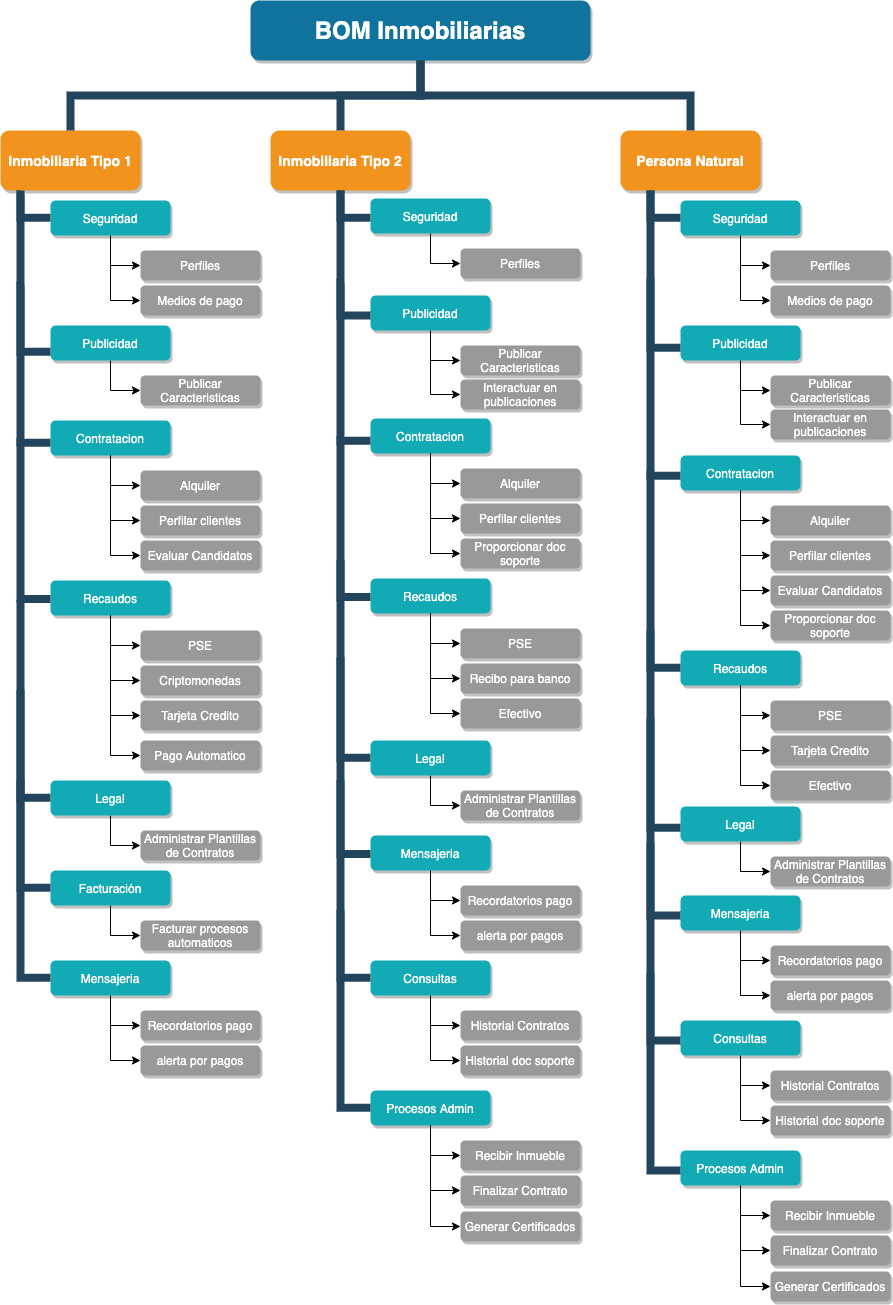
\includegraphics[scale=0.5]{images/BOM LP Inmobiliarias.png}
    \caption{Representación de productos de inmobiliaria para LP }
    \label{LPE}
\end{figure}
\FloatBarrier




%%%%%%%%%%%%%%%%%%%%%%%%%%%%%%%%%
% Julian
%%%%%%%%%%%%%%%%%%%%%%%%%%%%%%%%%
\section{\textbf{Evolución}}

La evolución de la linea de productos se plantea con respecto a los medios de pago disponibles para los diferentes segmentos de mercado permitiendo crecimiento vertical,  mixto y horizontal
\begin{itemize}
    \item Pago por PSE
    \item Pago con Tarjeta de Credito
    \item Pago con Cryptocurrencies
\end{itemize}

\begin{figure}[ht]
    \centering
    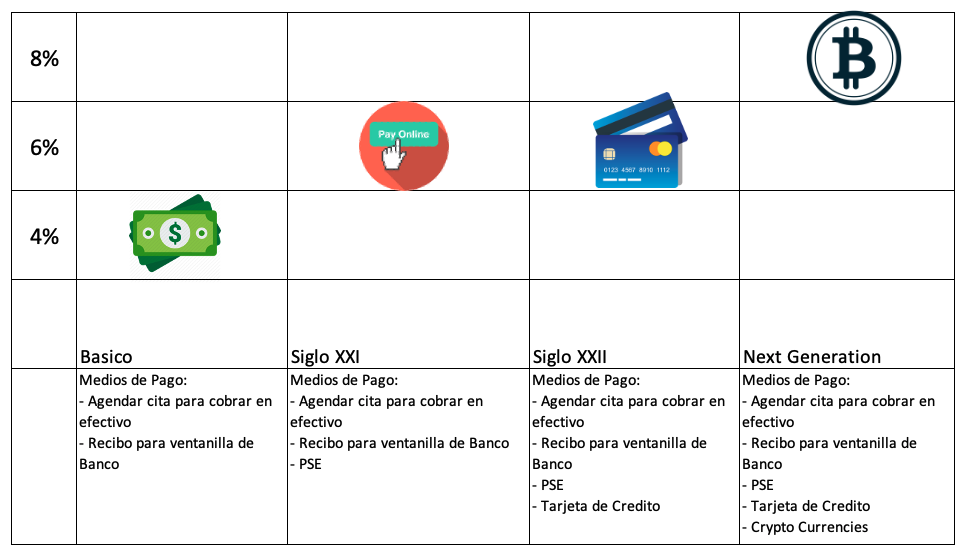
\includegraphics[scale=.5]{images/Evolucion LP.png}
    \caption{ Tabla de segmentos de mercado para el catálogo de App Inmobiliaria}
    \label{LPE}
\end{figure}
\FloatBarrier

Otros aspectos importantes que se evaluaran en las revisiones de la linea de productos son servicios agregados como:

\begin{itemize}
    \item Mantenimiento de inmuebles
    \item Reseñas de inquilinos
    \item Manejos de archivos asociados al contrato de arrendamiento
    \item Plantillas de contratos de arrendamiento
    \item Nuevos requerimientos comerciales de monetización
    \item Nuevos requerimientos introducidos por las normas legales y sus futuras actualizaciones 
\end{itemize}

\newpage

\section{\textbf{Arquitectura Propuesta}}

Se propone la siguiente arquitectura para una aplicación de inmobiliaria:

\begin{figure}[ht]
    \centering
    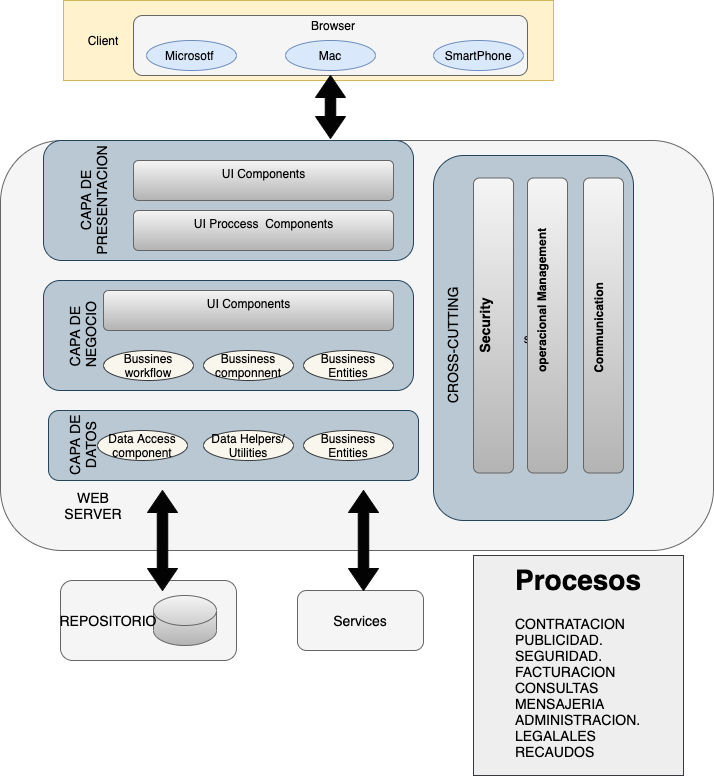
\includegraphics[width=5 in]{images/LPS.arqref.png}
    \caption{Arquitectura propuesta para App Inmobiliaria}
    \label{LPE}
\end{figure}
\FloatBarrier

\section{\textbf{Modelado de restricciones y validaciones.}}

Se propone el siguiente modelo de variabilidad para una aplicación de inmobiliaria dados los requerimientos funcionales establecidos (Se adjunta con este informe la tabla de requisitos de la linea de productos de inmobiliaria en un excel):
\begin{figure}[ht]
    \centering
    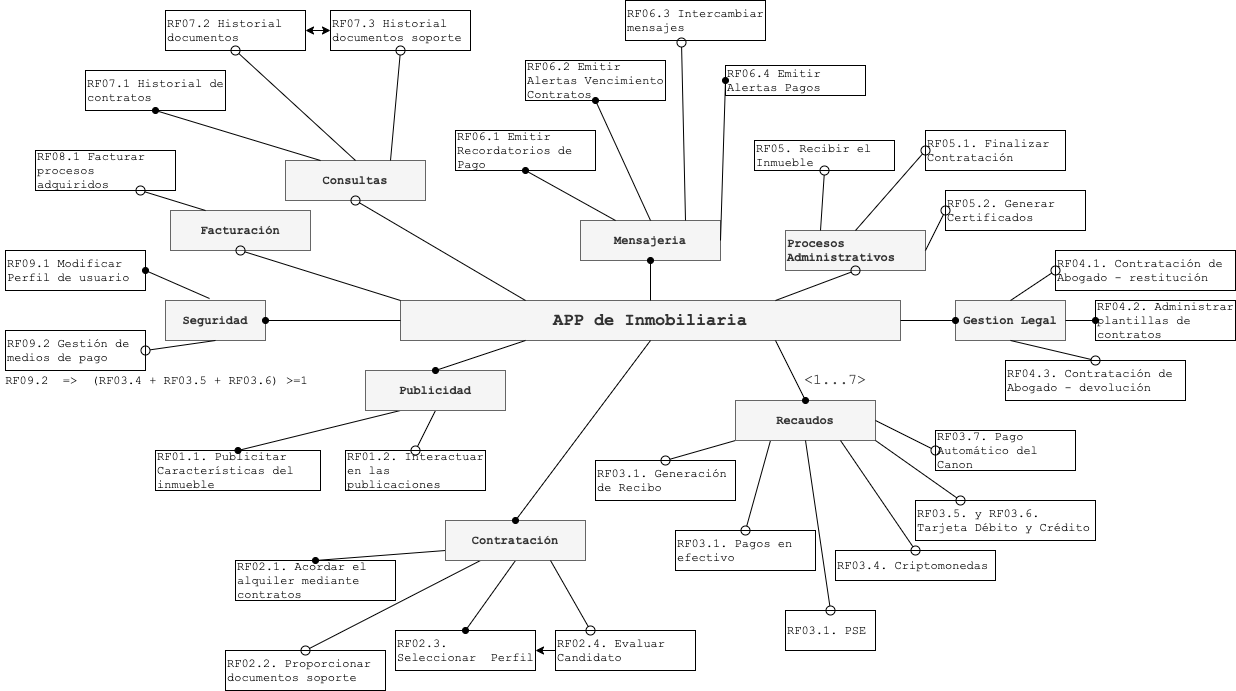
\includegraphics[width=6.8 in]{images/FM1.png}
    %\caption{ Tabla de segmentos de mercado para el catálogo de App Inmobiliaria}
    \label{LPE}
\end{figure}
\FloatBarrier

Se traduce el modelo de variabilidad a \href{https://github.com/ppsirg/puj-linea-producto/blob/main/inmueble.pl}{un modelo de restricciones} y con la herramienta GNU-Prolog se procede a realizar las siguientes validaciones. .

\begin{itemize}
    \item Validación de modelo vacío
    \item Validación de falso modelo de linea de productos
    \item Validación de variabilidad de los elementos variables
    \item Validación de elementos muertos
\end{itemize}

Para realizar las validaciones se desarrollaron una serie de \href{https://github.com/ppsirg/puj-linea-producto}{scripts disponibles en github} los cuales implementan las validaciones para sistematizar la revisión, para lo cual se obtuvieron los siguientes resultados:

\begin{verbatim}
(n4j) ->  linpro git:(main) - python -OO verifications.py
true product model
possible products:  1651968
RF5 designed as variable is variable
RF7 designed as variable is variable
RF8 designed as variable is variable
RF12 designed as variable is variable
RF22 designed as variable is variable
RF24 designed as variable is variable
RF31 designed as variable is variable
RF32 designed as variable is variable
RF33 designed as variable is variable
RF34 designed as variable is variable
RF35 designed as variable is variable
RF36 designed as variable is variable
RF37 designed as variable is variable
RF41 designed as variable is variable
RF43 designed as variable is variable
RF51 designed as variable is variable
RF52 designed as variable is variable
RF53 designed as variable is variable
RF63 designed as variable is variable
RF72 designed as variable is variable
RF73 designed as variable is variable
RF81 designed as variable is variable
RF92 designed as variable is variable
constant features:  ['F0', 'RF1', 'RF2', 'RF3', 'RF4', 'RF6', 'RF9', 'RF11', 
'RF21', 'RF23', 'RF42', 'RF61', 'RF62', 'RF64', 'RF71', 'RF91']

\end{verbatim}

Los resultados de la prueba muestran que el modelo es consistente en los aspectos ya verificados.


La prueba se realiza en un equipo Xubuntu 20.10 con python 3.7 y GNU Prolog 1.4.5, se observa que este tipo de analisis solo es factible para modelos pequeños debido a que el archivo de salida de GNU-prolog con todas las posibles combinaciones pesa al rededor de 100MB.



%ENTREGA 3 PROYECTO: IMPLEMENTACIONES DEL DOMINIO


%--NUEVA SECCION EN EL DOCUMENTO : CONFIGURACIONES DE LPS QUE INCLUYE
%--CONFIGURACIONES BASICAS (QUE QUIERO Y QUE NO ):  HACER CONFIGURACIONES DE NUESTRA LPS
%----QUE REQUISITOS SE OBTIENEN POR PROCESOS DE CONFIGURACIONES
%--CODIGO DE LOS COMPONENTES REUTILIZABLES DE DOMINIO
%--NO ES NECESARIO ESAMBLAR

\section{Implementaciones de Dominio}

\subsection{Configuraciones}

Se decide usar el enfoque guiado para la obtención de configuraciones, para ello se usa primero la heurística de las variables mas restringidas y luego la de las configuraciones de núcleo, para ello se detectan los requisitos incluidos en la mayor parte de restricciones, los cuales son:

\begin{itemize}
    \item RF34, RF35, RF36 (3 restricciones)
    \item RF72, RF73 (2 restricciones)
    \item RF23, RF24 (2 restricciones)
\end{itemize}

RF34 se refiere a recepción de pagos con criptomonedas mientras RF35 y RF36 se refieren a recepción de pagos con tarjeta débito y crédito respectivamente, por lo cual, tomando en consideración el uso de dichos medios de pago por parte del público objetivo y las barreras de entrada, tanto legales como comerciales, se toma la decisión de inhabilitar las características RF34 y RF35, la primera debido a la baja adopción del método de pago en el público objetivo de los productos pensados y el segundo porque dicho método de pago exige negociar banco por banco convenios de recaudación y en los diferentes países de la alianza del pacifico se necesitan códigos de recaudo, los cuales se dan a empresas con trayectoria y con grandes capitales de respaldo, y se decide dejar habilitado el requisito RF36 debido a que recientemente los países de la región han empezado a ofrecer productos de tarjeta de crédito con cero comisiones y desde plataforma digitales, lo que ha hecho que mucha gente bancarizada pueda acceder a productos como la tarjeta de crédito virtual recargable, dándose por ejemplo en el consumo de víveres, un \href{https://www.dinero.com/empresas/articulo/crecimiento-del-comercio-electronico-en-colombia-durante-la-pandemia/302658}{aumento de 7 por ciento el presente año}, ante lo que recibir pagos por este medio.

RF72 se refiere a tener un historial de documentos asociados y RF73 se refiere a tener un historial de documentos de soporte, debido a que son dos requisitos que pueden ser útiles a clientes muy especializados, se decide inhabilitarlos ambos.

Finalmente, los requisitos RF23 y RF24 aluden a la selección de perfil y la evaluación del candidato, debido a que un factor diferencial de nuestro producto es la asistencia a la toma de decisiones, se ha decidido habilitar ambos.

Luego del presente ejercicio, los requisitos con valores definidos son 

\begin{itemize}
    \item RF34 (inhabilitado), RF35 (inhabilitado), RF36 (habilitado)
    \item RF72 (inhabilitado), RF73 (inhabilitado)
    \item RF23 (habilitado), RF24 (habilitado)
\end{itemize}

Para aplicar la segunda heurística, se definen como características centrales las que se encuentran resaltadas en verde en el gráfico a continuación:

\begin{figure}
    \centering
    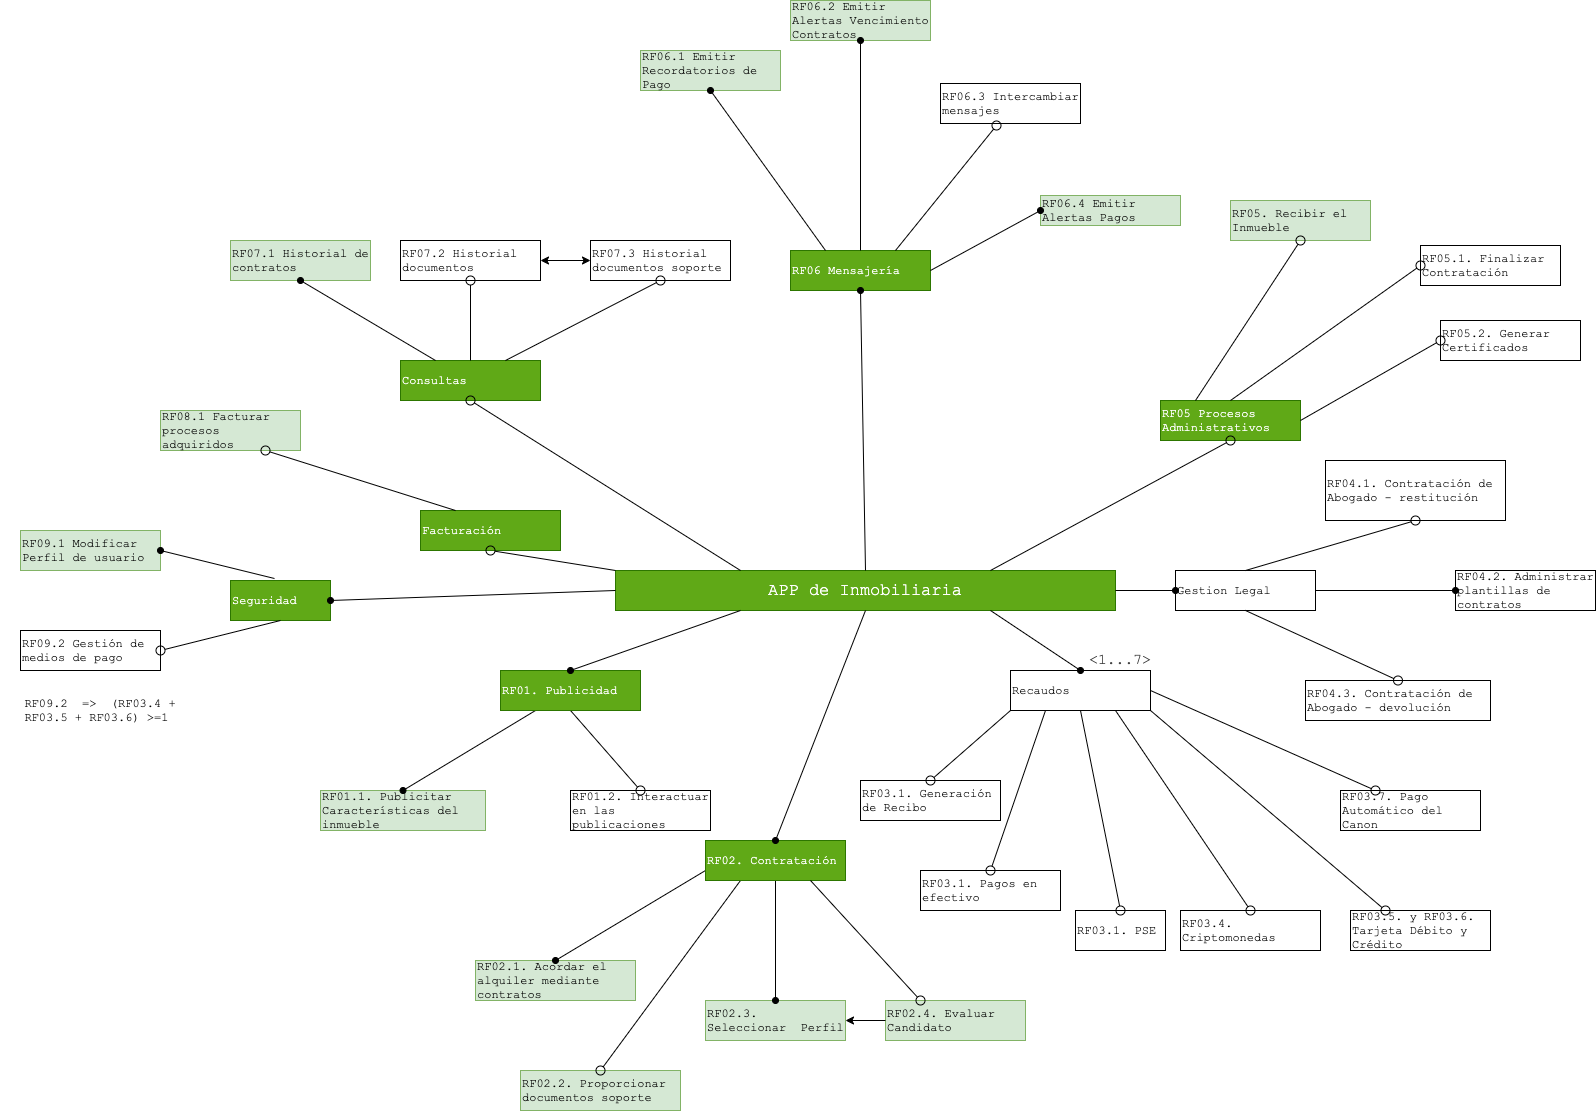
\includegraphics{images/reqprior.png}
    \caption{Características centrales para la familia de productos}
    \label{fig:core_feats}
\end{figure}

Con esto, se realiza una lista de los atributos centrales y los requisitos con más restricciones:

\begin{verbatim}
    marked = {
        # core first level
        "RF1": 1,
        "RF2": 1,
        "RF5": 1,
        "RF6": 1,
        "RF7": 1,
        "RF8": 1,
        "RF9": 1,
        # core sencond level
        "RF11": 1,
        "RF21": 1,
        "RF22": 1,
        "RF51": 1,
        "RF61": 1,
        "RF62": 1,
        "RF64": 1,
        "RF71": 1,
        "RF81": 1,
        "RF91": 1,
        # most constrained
        "RF34": 0,
        "RF35": 0,
        "RF36": 1,
        "RF72": 0,
        "RF73": 0,
        "RF23": 1,
        "RF24": 1,
    }
\end{verbatim}

Se ejecutan las nuevas restricciones salidas de la aplicación de las dos heurísticas en el solver para verificar que existan soluciones.

\begin{verbatim}
| ?- lpinmuebles(
     [_, 1, 1, _, _, 1, 1, 1, 1, 1, 1, _, 1, 1, 1, 1, _, _, _, 0, 0, 1, _, _, 
     _, _, 1, _, _, 1, 1, _, 1, 1, 0, 0, 1, 1, _]).

true ? 

yes
{1}
\end{verbatim}

y realizando nuevamente las revisiones de las variables faltantes, tenemos que los requisitos suceptibles de modifcarse en etapas posteriores son:

\begin{verbatim}
-> lineas python3 -OO verification.py
true product model
RF12 designed as variable is variable
RF31 designed as variable is variable
RF32 designed as variable is variable
RF33 designed as variable is variable
RF37 designed as variable is variable
RF41 designed as variable is variable
RF43 designed as variable is variable
RF52 designed as variable is variable
RF53 designed as variable is variable
RF63 designed as variable is variable
RF92 designed as variable is variable

variable_leaves
[
    "RF12",
    "RF31",
    "RF32",
    "RF33",
    "RF37",
    "RF41",
    "RF43",
    "RF52",
    "RF53",
    "RF63",
    "RF92",
]
\end{verbatim}

\newpage
\subsection{Arquitectura de Referencia}

\begin{figure}[ht]
    \centering
    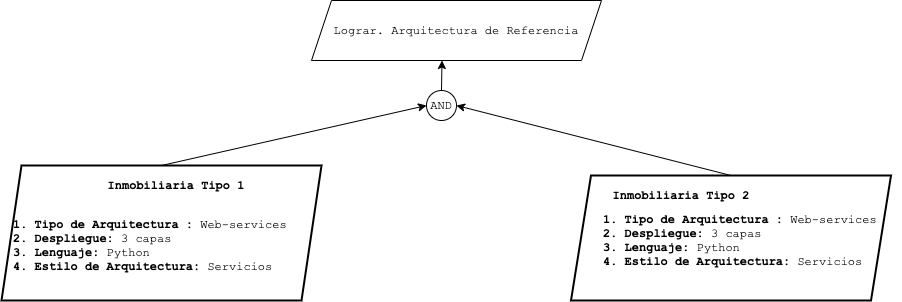
\includegraphics[width=3.5 in]{images/ARQR.png}
    \caption{Arquitectura de referencia para App Inmobiliaria}
    \label{LPE}
\end{figure}
\FloatBarrier

\subsubsection{Arquitectura modelo de componentes por producto}


\begin{figure}[ht]
    \centering
    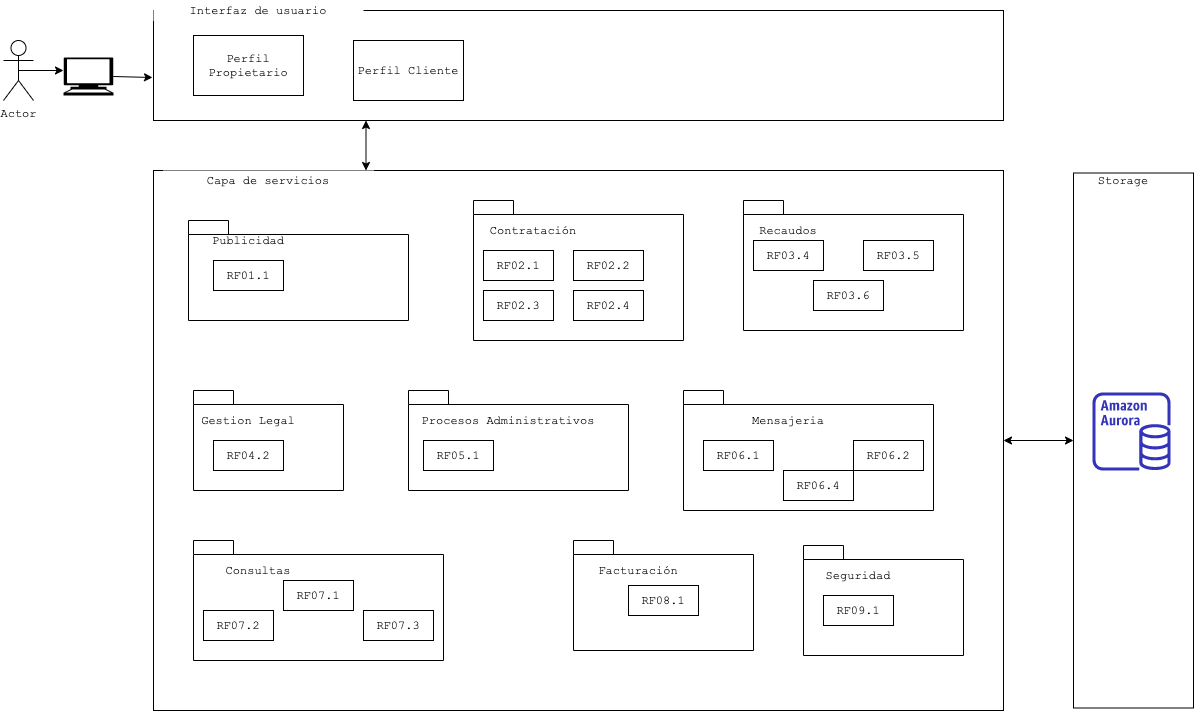
\includegraphics[width=3.6 in]{images/Tipo 1.png}
    \caption{Arquitectura para App Inmobiliaria Tipo 1}
    \label{LPE}
\end{figure}
\FloatBarrier


\begin{figure}[ht]
    \centering
    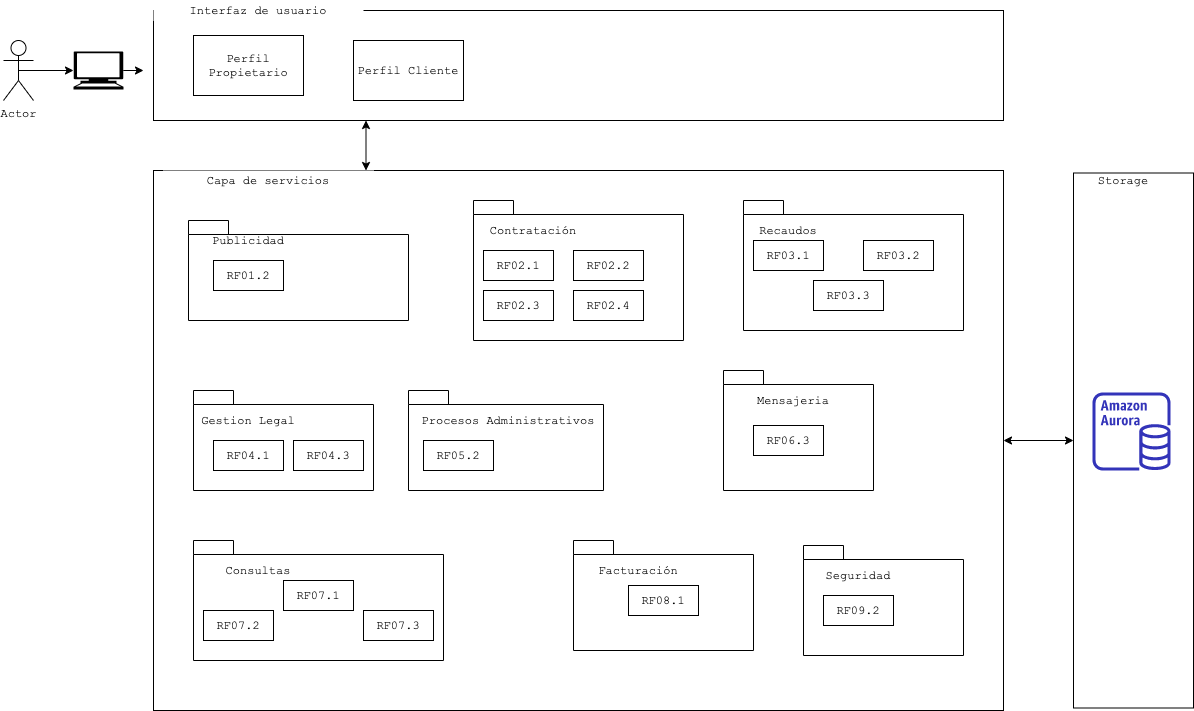
\includegraphics[width=3.6 in]{images/Tipo 2.png}
    \caption{Arquitectura para App Inmobiliaria Tipo 2}
    \label{LPE}
\end{figure}
\FloatBarrier


\end{document}

